\documentclass[10pt, pdf,xcolor=pdftex,dvipsnames,table]{beamer}

\usepackage[brazil]{babel}
\usepackage[utf8]{inputenc}
\usepackage[T1]{fontenc}

\usepackage{pgfpages}
%\usepackage{fancyvrb}
\usepackage{times}
%\usepackage{pgf,pgfarrows,pgfnodes,pgfautomata,pgfheaps}
\usepackage{amsmath,amssymb}
\usepackage{graphicx}
\usepackage{color}
\usepackage{hyperref}
\usepackage{pxfonts,txfonts}
\usepackage{url}
\usefonttheme{structurebold}
\usepackage{hyphenat}
\usepackage{multicol}
\usepackage{fp}
\usepackage{fancyvrb}
\usepackage{xcolor}
%\usepackage{enumitem}

\usepackage[caption=false]{subfig}
\usepackage{pgfplots}
\usepackage{pgfplotstable}
\usepackage{tikz}
\usetikzlibrary{patterns}

\definecolor{purpleheart}{rgb}{0.41, 0.21, 0.61}

\definecolor{airforceblue}{rgb}{0.36, 0.54, 0.66}

\definecolor{arylideyellow}{rgb}{0.91, 0.84, 0.42}

\definecolor{caribbeangreen}{rgb}{0.0, 0.8, 0.6}

\definecolor{cerulean}{rgb}{0.0, 0.48, 0.65}

\definecolor{terracotta}{rgb}{0.89, 0.45, 0.36}

\definecolor{tangelo}{rgb}{0.98, 0.3, 0.0}

\definecolor{dodgerblue}{rgb}{0.12, 0.56, 1.0}

\definecolor{tractorred}{rgb}{0.99, 0.05, 0.21}

\definecolor{brickred}{rgb}{0.8, 0.25, 0.33}

\definecolor{camouflagegreen}{rgb}{0.47, 0.53, 0.42}

%\usepackage{listings} % para inserir codigo fonte
%\lstset{extendedchars=true,
%breaklines=true,
%frame=tb,
%basicstyle=\footnotesize,
%stringstyle=\ttfamily,
%showstringspaces=false
%}

%\renewcommand{\lstlistingname}{Listagem}

\newcommand{\x}{\textbf{\textcolor{Green}{$\surd$}}}
\newcommand{\xx}{\textbf{\textcolor{Blue}{$\odot$}}}
\newcommand{\xxx}{\textbf{\textcolor{Red}{$\times$}}}

\newcommand{\tf}{\cellcolor{green!65}}
\newcommand{\tp}{\cellcolor{blue!65}}
\newcommand{\tn}{\cellcolor{yellow!65}}


% Comandos para auxiliar na construção de gráficos via latex

\usetheme{Amsterdam}
\setbeamertemplate{navigation symbols}{}

\pgfdeclareimage[height=1.5cm]{logo}{images/lups_oficial.png}
\logo{%
	%\hspace{5cm}
	%
\includegraphics[width=1cm,height=1cm,keepaspectratio]{images/lups_oficial.png}
	\hspace{5cm}
	\pgfuseimage{logo}
}

\setbeameroption{hide notes}

%==================================================================================

%EVENTO
\renewcommand{\evento}{Defesa de Mestrado}

% TITULO DA APRESENTACAO
\title{LTMS - Lups Transactional Memory Scheduler: Um escalonador NUMA-Aware para STM.}

%Autor
\author{\textbf{Michael Alexandre Costa}\\
\and Prof. Dr. André Rauber Du Bois (Orientador) \\
}

%%%%%%%%%%%%%%%%%%%%%%%%%%%%%%%%%%%%%%%%
% Instituição
%%%%%%%%%%%%%%%%%%%%%%%%%%%%%%%%%%%%%%%%

\institute{Mestrado em Computação \\ Centro de Desenvolvimento Tecnológico \\ Universidade Federal de Pelotas \\
\url{macosta@inf.ufpel.edu.br} 
}

\date{\today}

\begin{document}

% % % % % % % % % % % % % % % % % % % % % %
\frame{\titlepage}
\pgfdeclareimage[height=0.7cm]{logo}{images/lups_timbre.png}
\logo{%
	\pgfuseimage{logo}
}


% % % % % % % % % % % % % % % % % % % % % %
\frame{\tableofcontents}

%%%%%%%%%%%%%%%%%%%%%%%%%%%%%%%%%%%%%%%%%%%%%
% Conteúdo da Apresentação
%%%%%%%%%%%%%%%%%%%%%%%%%%%%%%%%%%%%%%%%%%%%%

\section{Introdução}

\begin{frame} \frametitle{Introdução}
    \begin{block}{Motivação}
        \begin{itemize}
        	\item Programação Paralela;
        	\item Memórias Transacionais;
        	\item Escalonadores de Transações; e
        	\item Arquiteturas NUMA.
        \end{itemize}
    \end{block}
\end{frame}

\begin{frame} \frametitle{Introdução}
    \begin{block}{Objetivos}
        \begin{itemize}
        	\item Projetar um escalonador de STM modular que considera a arquitetura utilizada, intitulado LTMS;
        	\item Prototipar o escalonador LTMS, utilizando a biblioteca de STM TinySTM; e
			\item Análisar de desempenho do LTMS comparado a TinySTM utilizando o conjunto de benchmarks STAMP.
        \end{itemize}
    \end{block}
\end{frame}

\section{Memórias Transacionais}

\begin{frame} \frametitle{Memórias Transacionais}
    \begin{block}{Características}
        \begin{itemize}
        	\item Fornece abstração de código;
        	\item Reuso de código; e
        	\item Ausência de deadlocks.
        \end{itemize}
    \end{block}
    
    \begin{block}{Transações}
        \begin{itemize}
        	\item Atomicidade;
        	\item Consistência; e
        	\item Isolamento.
        \end{itemize}
    \end{block}
\end{frame}

% \begin{frame} \frametitle{Memórias Transacionais}
%     \begin{block}{Controle das transações}
%         \begin{itemize}
%     		\item Versionamento de Dados:
%     		\begin{itemize}
%     			\item Adiantado / Tardio.
%     		\end{itemize}
%     		\item Detecção de Conflitos:
%     		\begin{itemize}
%     			\item Adiantado / Tardio.
%     		\end{itemize}
%     		\item Gerenciamento de Contenção:
%         		\begin{itemize}
%         		    \item Suicide, Delay, Backoff ou Modular.
%         		\end{itemize}
%         \end{itemize}
%     \end{block}
% \end{frame}

% \begin{frame} \frametitle{Memórias Transacionais}
% \begin{block}{Versionamento Adiantado}
% \begin{itemize}
% 	\item Escreve os dados especulativos direto na memória; e
% 	\item Em caso de um cancelamento, a operação deve ser desfeita.
% \end{itemize}
% % \begin{figure}[!h]
% % 	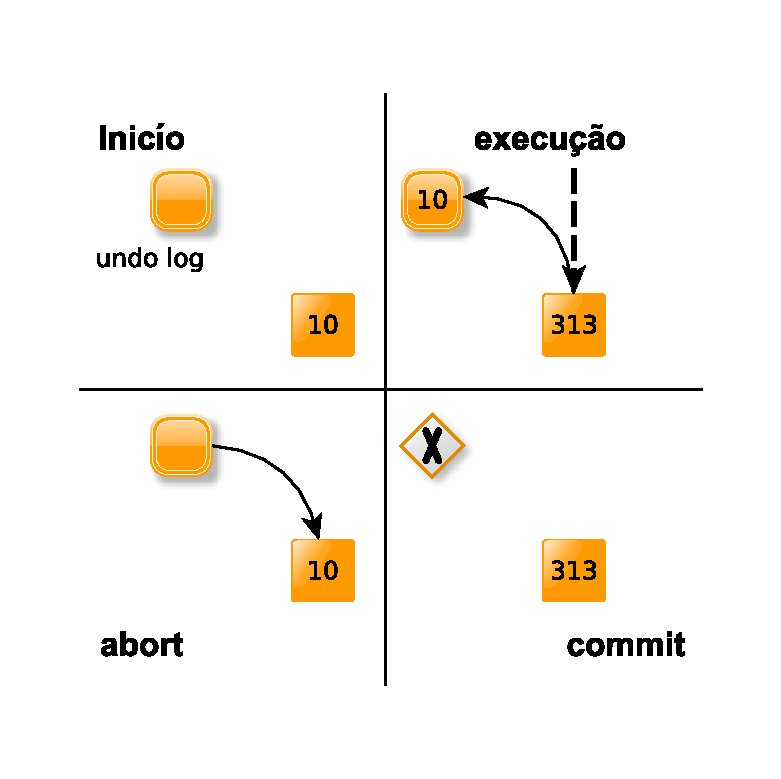
\includegraphics[scale=0.3]{images/versionamento_adiantado}
% % 	\caption{Versionamento Adiantado}
% % 	\label{fig:abusy}
% % \end{figure}
% \end{block}
% \begin{block}{Versionamento Tardio}
% \begin{itemize}
% 	\item Escreve os dados especulativos em um \textit{buffer} local; e
% 	\item Em caso de efetivação, os dados devem ser copiados para a memória.
% \end{itemize}
% % \begin{figure}[!h]
% % 	\centering
% % 	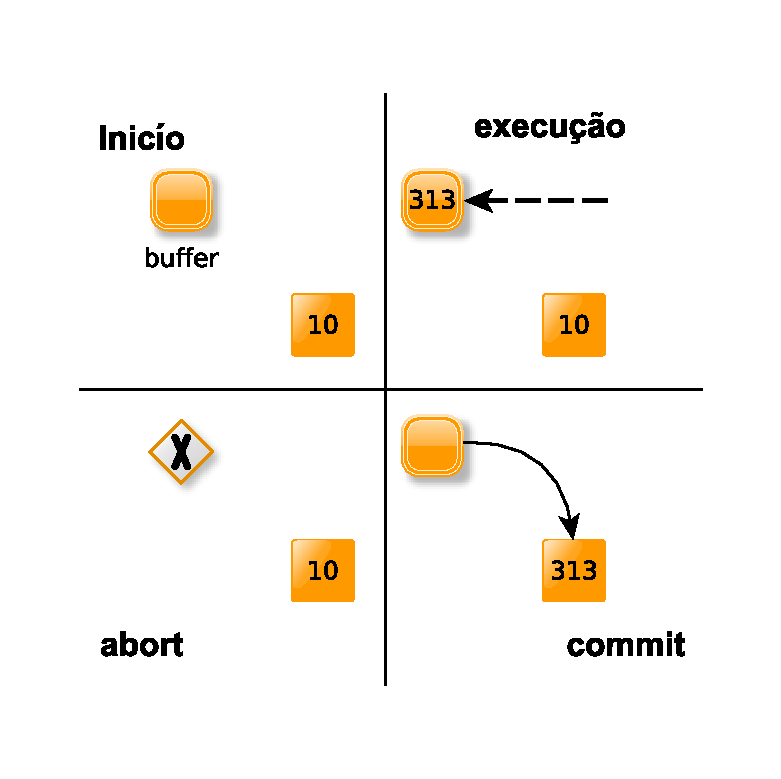
\includegraphics[scale=0.3]{images/versionamento_tardio}
% % 	\caption{Versionamento Tardio}
% % 	\label{fig:abusy}
% % \end{figure}
% % \begin{figure}[!h]
% % 	\centering
% % 	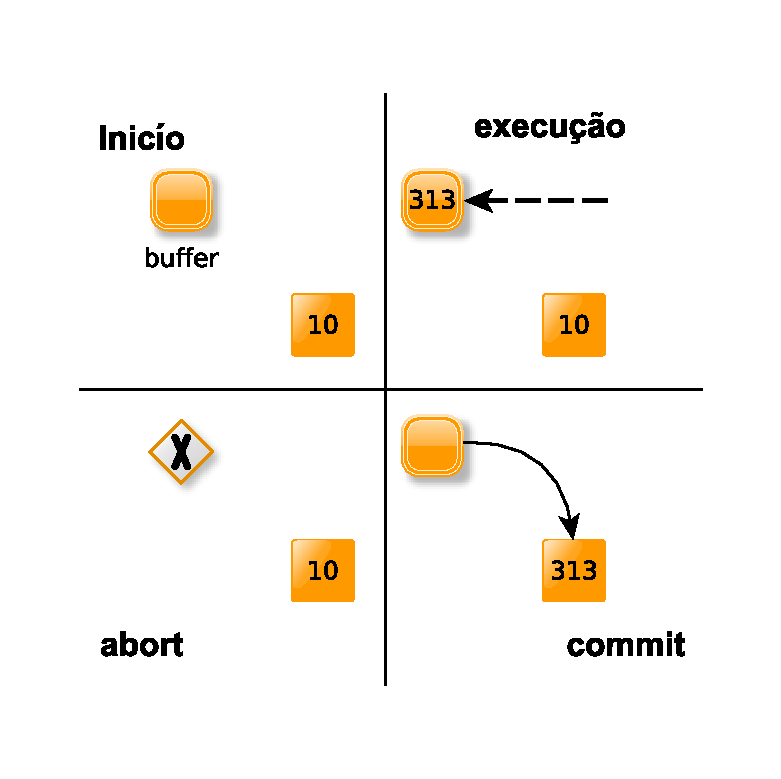
\includegraphics[scale=0.3]{images/versionamento_tardio}
% % 	\caption{Versionamento Tardio}
% % 	\label{fig:abusy}
% % \end{figure}
% \end{block}
% \end{frame}

% \begin{frame} \frametitle{Memórias Transacionais}
% \begin{block}{Detecção de Conflitos Adiantada}
% \begin{itemize}
% 	\item Detecta conflito no momento do acesso a memória.
% \end{itemize}
% % \begin{figure}[!h]
% % 	\centering	
% % 	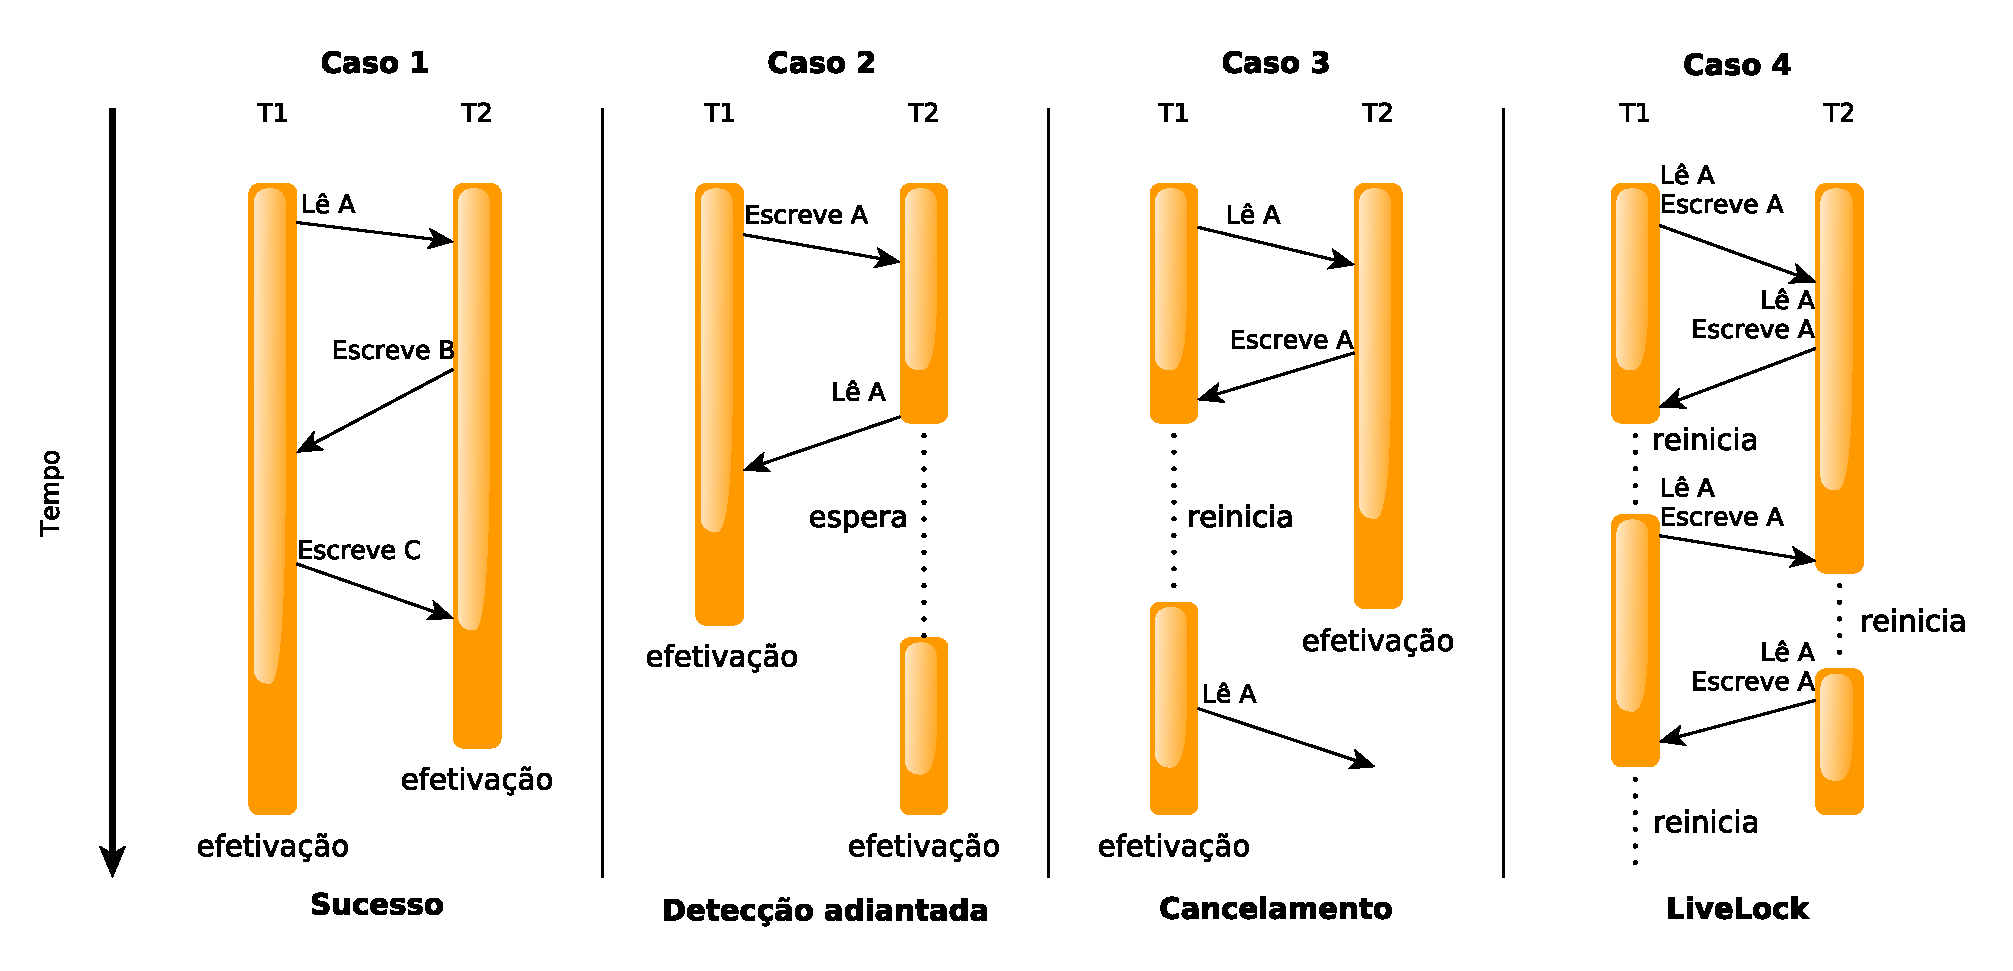
\includegraphics[scale=0.3]{images/deteccao_adiantada}
% % 	\caption{Detecção Adiantada}
% % 	\label{fig:abusy}
% % \end{figure}
% \end{block}
% \begin{block}{Detecção de Conflitos Tardia}
% \begin{itemize}
% 	\item Detecta conflito somente na validação.
% \end{itemize}
% % \begin{figure}[!h]
% % 	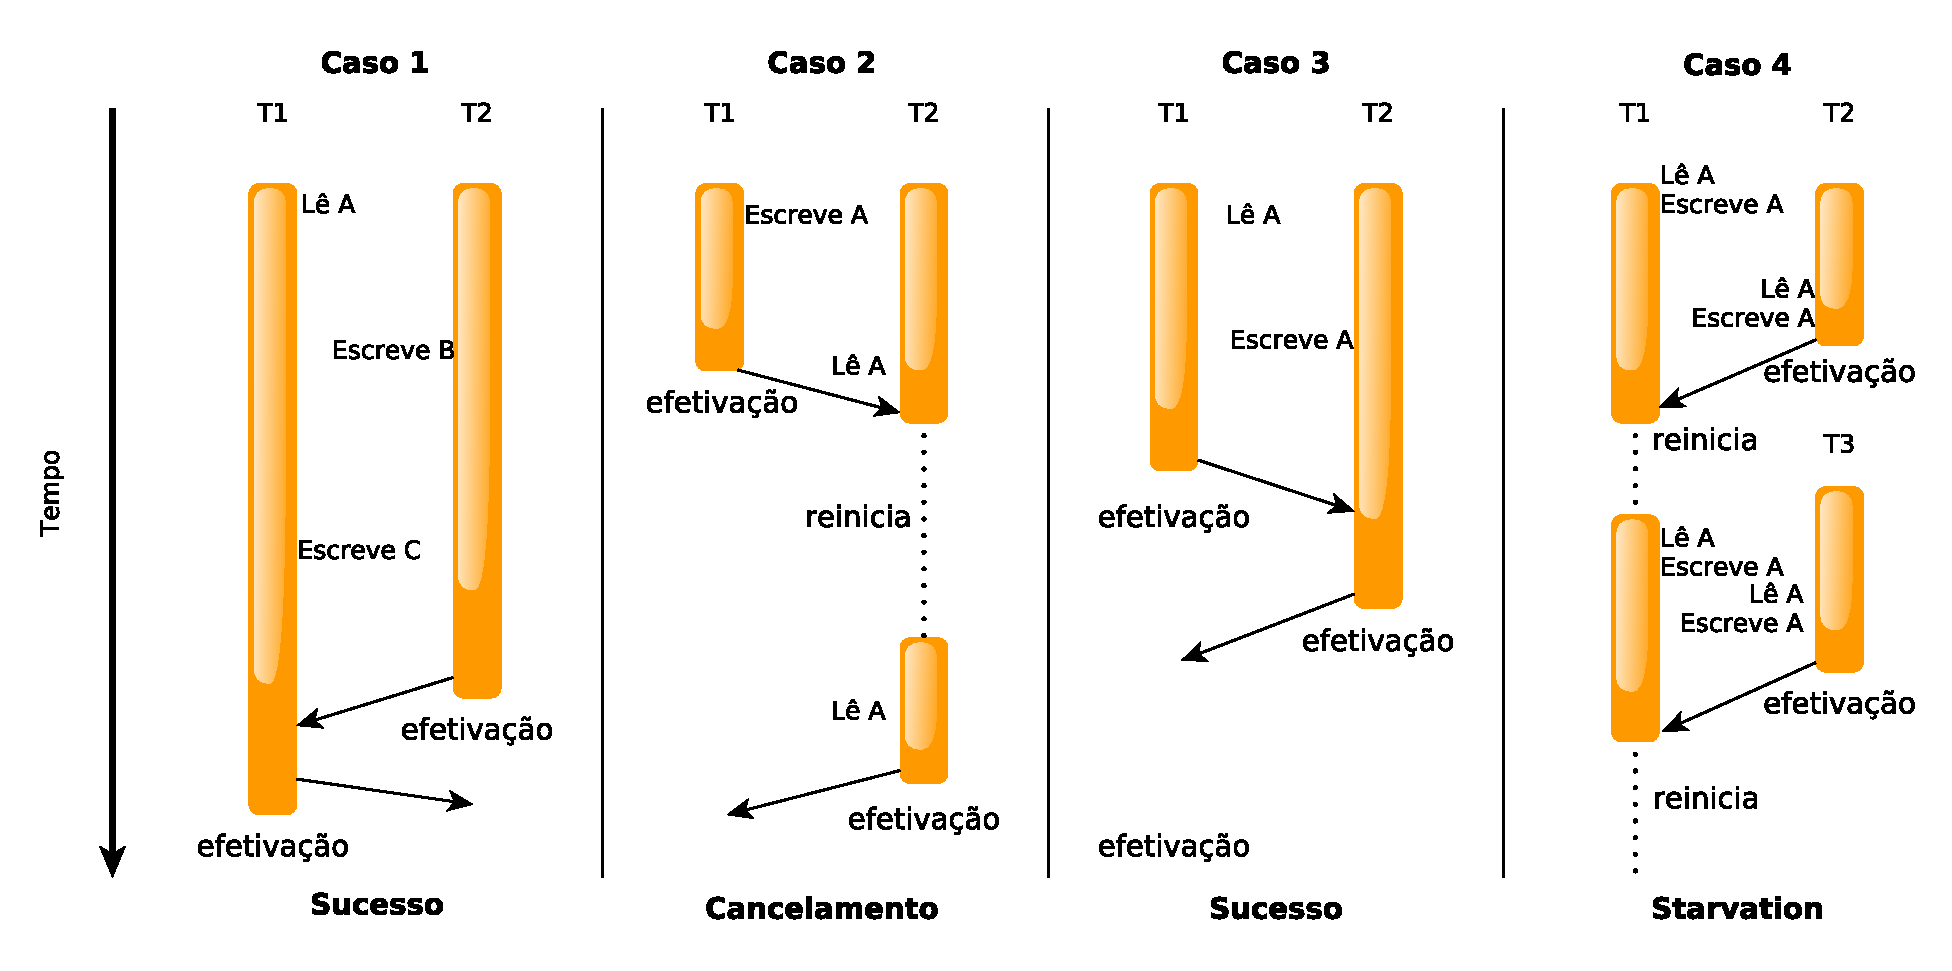
\includegraphics[scale=0.3]{images/deteccao_tardio}
% % 	\caption{Detecção Tardia}
% % 	\label{fig:abusy}
% % \end{figure}
% \end{block}
% \end{frame}

% \begin{frame} \frametitle{Memórias Transacionais}
%     \begin{block}{Gerenciador de Contenção}
%         \begin{itemize}
%         	\item Possui ação reativa;
%         	\item Suicide, Delay, Backoff ou Modular.
%         % 	\begin{itemize}
%         % 	    \item Suicide, Delay, Aggressive, e Timestamp.
%         %     \end{itemize}
%         \end{itemize}
%     \end{block}
%     \begin{block}{Gerenciador de Contenção}
%         \begin{itemize}
%             \item Modular:
%             \begin{itemize}
%     	        \item Suicide, Delay, Aggressive, e Timestamp.
%             \end{itemize}
%         \end{itemize}
%     \end{block}
%     % \begin{alertblock}{Problemas}
%     %     \begin{itemize}
%     %     	\item Somente reinicia a transação conflitante;
%     %     	\item Não evita que conflitos futuros aconteçam; e
%     %     	\item Em ambientes de alta contenção, tende a perder desempenho.
%     %     \end{itemize}
%     % \end{alertblock}
% \end{frame}

\begin{frame} \frametitle{Memórias Transacionais}
    % \begin{block}{Gerenciador de Contenção}
    %     \begin{itemize}
    %     	\item Possui ação reativa;
    %     	\item Suicide, Delay, Backoff ou Modular.
    %     % 	\begin{itemize}
    %     % 	    \item Suicide, Delay, Aggressive, e Timestamp.
    %     %     \end{itemize}
    %     \end{itemize}
    % \end{block}
    % \begin{block}{Modular}
    %     \begin{itemize}
    % 	    \item Suicide, Delay, Aggressive, e Timestamp.
    %     \end{itemize}
    % \end{block}
    \begin{alertblock}{Problemas}
        \begin{itemize}
        	\item Somente reinicia a transação conflitante;
        	\item Não evita que conflitos futuros aconteçam; e
        	\item Em ambientes de alta contenção, tende a perder desempenho.
        \end{itemize}
    \end{alertblock}
\end{frame}

\section{Escalonadores}
\begin{frame} \frametitle{Escalonadores}
\begin{block}{Escalonadores de Transações}
\begin{itemize}
	\item Buscam reduzir os números de conflitos;
	\item Utilizam diferentes Heurísticas de escalonamento; e
	\item Serializa as transações conflitantes.
\end{itemize}
\end{block}
\end{frame}

\begin{frame} \frametitle{Escalonadores}
\begin{block}{Classificação das técnicas}
\begin{itemize}
	\item Baseado em Heurística:
	\begin{itemize}
	    \item Feedback;
	    \item Predição;
	    \item Reativo; e
	    \item Heurística Mista.
	\end{itemize}
	\item Baseado em Modelo:
	\begin{itemize}
	    \item Aprendizado de Máquina;
	    \item Modelo Analítico; e
	    \item Modelo Misto.
	\end{itemize}
\end{itemize}
\end{block}
\end{frame}


\begin{frame} \frametitle{Escalonadores}
\begin{block}{Trabalhos Relacionados}
\begin{table}[]
\footnotesize
\centering
\caption{Algoritmos e técnicas de escalonamento}
\label{tab:compare}
\begin{tabular}{l|l}
\hline
Escalonador & Técnica \\ \hline
ATS & Feedback \\
Probe & Feedback \\
F2C2 & Feedback \\
Shrink & Predição \\
SCA & Predição \\
CAR-STM & Reativo \\
RelSTM & Reativo \\
LUTS & Heurística Mista \\
ProVIT & Heurística Mista \\
SAC-STM & Aprendizado de Máquina \\
CSR-STM & Modelo Analítico \\
MCATS & Modelo Analítico \\
AML & Modelo Misto \\
\hline
\end{tabular}
\end{table}
\end{block}
\end{frame}

\begin{frame} \frametitle{Escalonadores}
\begin{block}{Trabalhos Relacionados}
\begin{table}[]
\footnotesize
\centering
\caption{Algoritmos que estamos trabalhando}
\label{tab:compare}
\begin{tabular}{l|l}
\hline
Escalonador & Técnica \\ \hline
Probe & Feedback \\
F2C2 & Feedback \\
Shrink & Predição \\
MCATS & Modelo Analítico \\
\hline
\end{tabular}
\end{table}
\end{block}
\end{frame}

% \begin{frame} \frametitle{Escalonadores}
% \begin{block}{Shrink}
% \begin{itemize}
%     \item Bloom filter: Utiliza os dados de leitura e escrita por thread:
%     \begin{itemize}
%         \item Conjunto de leitura: Localidade temporal; e
%         \item Conjunto de escrita: Ocorre apenas nos aborts.
%     \end{itemize}
%     \item Serialization affinity: Serializa uma thread de acordo com a contenção do sistema; e
%     \item O escalonador é ativado com base no número de contenção existente.
% \end{itemize}
% \end{block}
% \end{frame}

\section{Arquiteturas}
\begin{frame} \frametitle{Arquiteturas}
\begin{block}{UMA}
\begin{itemize}
	\item Uniform Memory access;
	\item Possui um único barramento de acesso à memória; e
	\item Único custo de acesso à memória.
\end{itemize}
\end{block}
\begin{block}{NUMA}
\begin{itemize}
	\item Non-uniform Memory access;
	\item Possui mais de um barramento de acesso à memória; e
	\item O custo de acesso à memória é diferente conforme o núcleo utilizado.
\end{itemize}
\end{block}
\end{frame}

\section{LTMS}
\begin{frame} \frametitle{LTMS}
    \begin{block}{Estágios}
        \begin{itemize}
        	\item Inicialização do sistema;
        	\item Coleta de dados em tempo de execução; e
        	\item Migração de Threads.
        \end{itemize}
    \end{block}
\end{frame}

\begin{frame} \frametitle{LTMS}
    \begin{block}{Escalonador}
        \begin{itemize}
        	\item imagem
        \end{itemize}
    \end{block}
\end{frame}

\begin{frame} \frametitle{LTMS - Estágio 1}
    \begin{block}{Inicialização do sistema}
        \begin{itemize}
        	\item Criação de filas; e
        	\item Distribuição das threads.
        \end{itemize}
    \end{block}

    \begin{block}{Heurísticas de Distribuição}
        \begin{itemize}
        	\item Sequential; e
        	\item Chunks.
        \end{itemize}
    \end{block}
\end{frame}

\begin{frame} \frametitle{LTMS - Heurísticas}
    \begin{figure}[!h]
        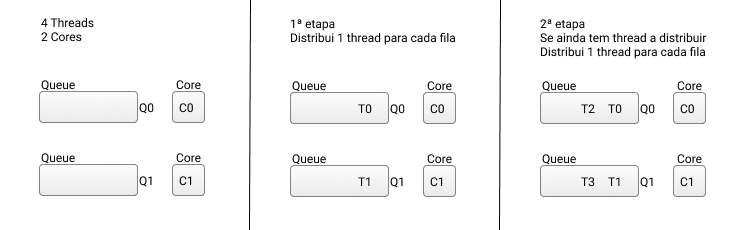
\includegraphics[scale=0.4]{images/Queue_one}
        \caption{Heurística Sequential}
        \label{fig:abusy}
    \end{figure}
\end{frame}

\begin{frame} \frametitle{LTMS- Heurísticas}
    \begin{figure}[!h]
        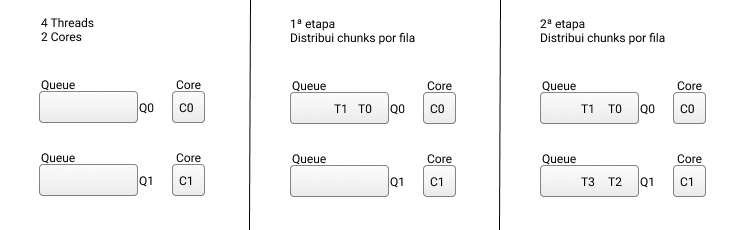
\includegraphics[scale=0.4]{images/Queue_chunks}
        \caption{Heurística Chunks}
        \label{fig:abusy}
    \end{figure}
\end{frame}

\begin{frame} \frametitle{LTMS - Estágio 2}
    \begin{block}{Coleta de dados em tempo de execução}
        \begin{itemize}
        	\item Aborts e Commits;
        	\item Matriz de Comunicação; e 
        	\item Matriz de Endereços.
        \end{itemize}
    \end{block}
\end{frame}

\begin{frame} \frametitle{LTMS - Matrizes}
    \begin{block}{Matriz de Comunicação}
        \begin{itemize}
        	\item Quantidade de comunicação entre pares de threads;
        	\item Eventos de Comunicação; e
        	\item 1 evento a cada 100 acessos.
        \end{itemize}
    \end{block}
    % A matriz de comunicação fornece insumos sobre a quantidade eventos de comunicação entre dois threads, onde cada posição da matriz representa a quantidade de comunicação entre pares de threads.
\end{frame}

\begin{frame} \frametitle{LTMS - Matrizes}
    \begin{block}{Matriz de Endereços}
        \begin{itemize}
        	\item Endereço mais acessado entre pares de threads;
        	\item Tabela Hash;
        	\item Endereços de memória; e 
            \item Quantidade de acessos recebidos.
        \end{itemize}
        % possui para cada posição uma tabela hash que contem uma estrutura de chave e valor. Esta estrutura utiliza como chave o endereço de memória acessado e como valor, a quantidade de acessos que este endereço recebeu.Quando duas threds acessam o mesmo endereço de memória, um evento é disparado, este evento busca na tabela hash a chave com endereço que foi acessado e incrementa o valor de acessos que este endereço recebeu.
    \end{block}
\end{frame}

\begin{frame} \frametitle{LTMS - Estágio 3}
    \begin{block}{Migração de Threads}
        \begin{itemize}
        	\item Abort;
        	\item Identificação; e
            \item Heurísticas de migração.
        \end{itemize}
    \end{block}
\end{frame}

\begin{frame} \frametitle{LTMS - Filas e Threads}
    \begin{block}{Identificação das filas e threads}
        \begin{itemize}
        	\item Identificação das threads conflitantes; e
        	\item Matriz de comunicação.
        \end{itemize}
    \end{block}
    % A etapa de identificação das threads conflitantes busca entender a aplicação e a arquitetura para definir para qual fila a thread que gerou o abort deve ser migrada.
\end{frame}

\begin{frame} \frametitle{LTMS - Heurísticas}
    \begin{block}{Threshold}
        \begin{itemize}
        	\item Nível de contenção (Abort/Commit);
        	\item Maior contenção;
        	\item Menor contenção; e
        	\item Limiar de 0.8 (80\% de contenção).
        \end{itemize}
    \end{block}
\end{frame}

\begin{frame} \frametitle{LTMS - Heurísticas}
    \begin{block}{Latency}
        \begin{itemize}
        	\item Matriz de endereços;
        	\item Nodos NUMA;
        	\item Bancos de memória; e
        	\item Latencia.
        \end{itemize}
    \end{block}
\end{frame}

\section{Experimentos}
\begin{frame} \frametitle{Experimentos}
    \begin{block}{Aplicação}
        \begin{itemize}
            \item TinySTM 1.0.5; e
            \item STMAP 0.9.10.
        \end{itemize}
    \end{block}
 
    \begin{block}{Arquitetura}
        \begin{itemize}
        	\item Intel Xeon E5-4650;
            \item 96 núcleos e 192 threads;
            \item 468Gb de memória RAM.
        \end{itemize}
    \end{block}
\end{frame}

\begin{frame} \frametitle{Experimentos}
    \begin{block}{Testes}
        \begin{itemize}
        	\item Cenários de threads: 
            \begin{itemize}
                \item 1, 2, 4, 8, 16, 32, 64, 128, 256, e 512;
            \end{itemize}
            \item Heurísticas de Distribuição-Migração:
            \begin{itemize}
                \item Sequential-Threshold;
                \item Chunks-Threshold;
                \item Sequential-Latency;
                \item Chunks-Latency;
            \end{itemize}
            \item TinySTM; e
            \item Baterias de 30 execuções.
        \end{itemize}
    \end{block}
\end{frame}

\section{Resultados}
\begin{frame} \frametitle{Resultados}
    \begin{block}{Benchmarks}
        \begin{itemize}
        	\item Bayes;
        	\item Intruder;
        	\item Kmeans; e
        	\item Labyrinth, Vacation, Yada.
        \end{itemize}
    \end{block}
\end{frame}

\begin{frame} \frametitle{Tempo de execução}
    \begin{figure}[!ht]
    \centering
    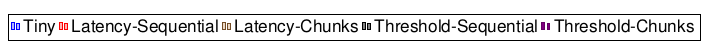
\includegraphics[scale=0.3]{images/legend}
    
    \subfloat[Intruder]{
        \label{Intruder}
        \begin{tikzpicture}[scale=0.35, baseline]
        \begin{axis}[
            width=1.5 \linewidth,
            height=1 \linewidth,
            %media de tempo intruder
            ybar=2.5pt,
            % enlargelimits=0.10,
            % legend style={at={(0.45,1.1)}, anchor=south, legend columns=0, nodes={scale=2}},
            ylabel=Tempo(s),
            xlabel=Threads,
            symbolic x coords={1, 2, 4, 8, 16, 32, 64, 128, 256, 512},
            xtick=data,
            ymin=0,
            ymax=400,
            bar width=5pt,
            % nodes near coords,
            nodes near coords align={vertical},
        ]
        \addplot+[error bars,y dir=both, y explicit] coordinates {
            (1,22.49)+-(1,0.11) (2,47.47)+-(2,0.69) (4,36.62)+-(4,0.59) (8,39.90)+-(8,0.89) (16,40.47)+-(16,0.35) (32,40.54)+-(32,3.55) (64,42.59)+-(64,0.29) (128,47.43)+-(128,1.97) (256,122.18)+-(256,4.64) (512,356.05)+-(512,5.11) 
        };
        \addplot+[error bars,y dir=both, y explicit] coordinates {
            (1,27.06)+-(1,0.18) (2,16.76)+-(2,0.13) (4,11.43)+-(4,0.10) (8,8.18)+-(8,0.13) (16,7.20)+-(16,0.06) (32,7.31)+-(32,0.14) (64,8.25)+-(64,0.81) (128,8.00)+-(128,0.37) (256,10.82)+-(256,3.29) (512,11.20)+-(512,0.86)
        };
        \addplot+[error bars,y dir=both, y explicit] coordinates {
            (1,26.90)+-(1,0.17) (2,16.89)+-(2,0.13) (4,11.50)+-(4,0.13) (8,8.10)+-(8,0.10) (16,7.21)+-(16,0.06) (32,7.28)+-(32,0.07) (64,7.61)+-(64,0.63) (128,9.11)+-(128,0.98) (256,10.40)+-(256,2.68) (512,11.59)+-(512,0.72)
        };
        \addplot+[error bars,y dir=both, y explicit] coordinates {
            (1,27.73)+-(1,0.05) (2,16.65)+-(2,0.16) (4,10.50)+-(4,1.10) (8,6.64)+-(8,0.23) (16,24.42)+-(16,2.56) (32,29.00)+-(32,6.41) (64,28.59)+-(64,10.33) (128,25.01)+-(128,0.29) (256,26.19)+-(256,1.25) (512,27.87)+-(512,2.82)
        };
        \addplot+[error bars,y dir=both, y explicit] coordinates {
            (1,27.96)+-(1,0.25) (2,28.12)+-(2,0.28) (4,28.11)+-(4,0.14) (8,28.17)+-(8,0.07) (16,23.01)+-(16,1.76) (32,36.20)+-(32,1.18) (64,30.24)+-(64,4.39) (128,24.97)+-(128,1.10) (256,26.99)+-(256,2.13) (512,27.18)+-(512,2.84)
        };
        % \legend {Tiny, Latency-Sequential, Latency-Chunks, Threshold-Sequential, Threshold-Chunks}
        \end{axis}
        \end{tikzpicture}
    }
    \subfloat[Kmeans]{
        \label{Kmeans}
        \begin{tikzpicture}[scale=0.35, baseline]
        \begin{axis}[
            width=1.5 \linewidth,
            height=1 \linewidth,
            %media de tempo intruder
            ybar=2.5pt,
            %enlargelimits=0.10,
            % legend style={at={(0.5,-0.15)}, anchor=north, legend columns=-1},
            ylabel=Tempo(s),
            xlabel=Threads,
            symbolic x coords={1, 2, 4, 8, 16, 32, 64, 128, 256, 512},
            xtick=data,
            ymin=0,
            ymax=150,
            bar width=5pt,
            % nodes near coords,
            nodes near coords align={vertical},
        ]
        \addplot+[error bars,y dir=both, y explicit] coordinates {
            (1,13.32)+-(1,0.05) (2,18.64)+-(2,1.86) (4,15.33)+-(4,2.68) (8,14.72)+-(8,2.44) (16,12.06)+-(16,0.95) (32,18.24)+-(32,5.19) (64,20.20)+-(64,7.21) (128,32.16)+-(128,15.30) (256,40.54)+-(256,4.28) (512,81.86)+-(512,19.67) 
        };
        \addplot+[error bars,y dir=both, y explicit] coordinates {
            (1,13.36)+-(1,0.05) (2,8.25)+-(2,1.41) (4,5.05)+-(4,0.53) (8,3.49)+-(8,0.45) (16,8.10)+-(16,1.15) (32,25.81)+-(32,4.77) (64,14.01)+-(64,1.61) (128,19.77)+-(128,3.11) (256,34.76)+-(256,10.90) (512,105.07)+-(512,0.66)
        };
        \addplot+[error bars,y dir=both, y explicit] coordinates {
            (1,13.39)+-(1,0.03) (2,8.05)+-(2,1.09) (4,5.13)+-(4,0.64) (8,3.37)+-(8,0.57) (16,7.62)+-(16,1.79) (32,13.01)+-(32,3.05) (64,21.35)+-(64,3.62) (128,21.05)+-(128,7.45) (256,57.98)+-(256,27.06) (512,103.22)+-(512,3.24)
        };
        \addplot+[error bars,y dir=both, y explicit] coordinates {
            (1,13.70)+-(1,0.00) (2,8.08)+-(2,0.39) (4,6.03)+-(4,1.01) (8,2.85)+-(8,0.20) (16,7.92)+-(16,1.01) (32,14.57)+-(32,1.81) (64,19.24)+-(64,2.21) (128,18.49)+-(128,0.48) (256,52.31)+-(256,2.27) (512,111.88)+-(512,4.66) 
        };
        \addplot+[error bars,y dir=both, y explicit] coordinates {
            (1,13.73)+-(1,0.00) (2,13.72)+-(2,0.00) (4,14.49)+-(4,0.02) (8,8.98)+-(8,3.78) (16,15.66)+-(16,2.82) (32,12.59)+-(32,0.01) (64,16.86)+-(64,1.83) (128,21.99)+-(128,1.45) (256,24.41)+-(256,0.44) (512,119.27)+-(512,3.89)
        };
        % \legend {Tiny, Latency-Sequential, Latency-Chunks, Threshold-Sequential, Threshold-Chunks}
        \end{axis}
        \end{tikzpicture}
    }
\end{figure}

\end{frame}

\begin{frame} \frametitle{Tempo de execução}
    \begin{figure}[!ht]
    % \centering
    \subfloat[Labyrinth]{
        \label{Labyrinth}
        \begin{tikzpicture}[scale=0.35, baseline]
            \begin{axis}[
                width=1.5 \linewidth,
                height=1 \linewidth,
                %media de tempo intruder
                ybar=2.5pt,
                %enlargelimits=0.10,
                legend style={at={(0.45,1.1)}, anchor=south, legend columns=-1},
                ylabel=Tempo(s),
                xlabel=Threads,
                symbolic x coords={1, 2, 4, 8, 16, 32, 64, 128, 256, 512},
                xtick=data,
                ymin=0,
                ymax=600,
                bar width=5pt,
                % nodes near coords,
                nodes near coords align={vertical},
            ]
            \addplot+[error bars,y dir=both, y explicit] coordinates {
                (1,543.12)+-(1,0.14) (2,307.12)+-(2,3.77) (4,177.18)+-(4,3.79) (8,86.06)+-(8,0.82) (16,50.63)+-(16,0.60) (32,35.89)+-(32,0.53) (64,26.45)+-(64,0.63) (128,25.83)+-(128,0.64) (256,41.98)+-(256,1.85) (512,57.32)+-(512,2.08) 
            };
            \addplot+[error bars,y dir=both, y explicit] coordinates {
                (1,553.57)+-(1,0.26) (2,287.70)+-(2,0.17) (4,165.86)+-(4,0.67) (8,94.13)+-(8,1.50) (16,65.04)+-(16,2.20) (32,37.22)+-(32,1.17) (64,25.60)+-(64,1.00) (128,25.49)+-(128,1.49) (256,26.10)+-(256,1.15) (512,25.80)+-(512,0.75)
            };
            \addplot+[error bars,y dir=both, y explicit] coordinates {
                (1,553.49)+-(1,0.21)(2,287.57)+-(2,0.25)(4,165.74)+-(4,0.99)(8,93.35)+-(8,1.29)(16,65.67)+-(16,6.11)(32,38.25)+-(32,1.76)(64,29.61)+-(64,0.77)(128,26.85)+-(128,2.24)(256,25.63)+-(256,0.42)(512,27.96)+-(512,1.35)
            };
            \addplot+[error bars,y dir=both, y explicit] coordinates {
                (1,553.89)+-(1,0.08) (2,287.30)+-(2,0.32) (4,164.88)+-(4,0.69) (8,93.33)+-(8,0.76) (16,55.06)+-(16,0.46) (32,35.27)+-(32,0.97) (64,26.35)+-(64,1.17) (128,26.33)+-(128,1.74) (256,26.96)+-(256,1.43) (512,29.70)+-(512,2.27) 
            };
            \addplot+[error bars,y dir=both, y explicit] coordinates {
                (1,553.38)+-(1,0.02) (2,287.58)+-(2,0.22) (4,164.99)+-(4,0.38) (8,93.83)+-(8,0.15) (16,55.92)+-(16,0.76) (32,35.17)+-(32,0.71) (64,26.79)+-(64,0.74) (128,25.67)+-(128,0.66) (256,27.99)+-(256,1.60) (512,28.01)+-(512,0.74)
            };
        \legend {Tiny, Latency-Sequential, Latency-Chunks, Threshold-Sequential, Threshold-Chunks}
        \end{axis}
        \end{tikzpicture}
    }
    \subfloat[Vacation]{
        \label{Vacation}
        \begin{tikzpicture}[scale=0.35, baseline]
        \begin{axis}[
            width=1.5 \linewidth,
            height=1 \linewidth,
            %media de tempo intruder
            ybar=2.5pt,
            %enlargelimits=0.10,
            % legend style={at={(0.5,-0.15)}, anchor=north, legend columns=-1},
            ylabel=Tempo(s),
            xlabel=Threads,
            symbolic x coords={1, 2, 4, 8, 16, 32, 64, 128, 256, 512},
            xtick=data,
            ymin=0,
            ymax=200,
            bar width=5pt,
            % nodes near coords,
            nodes near coords align={vertical},
        ]
        \addplot+[error bars,y dir=both, y explicit] coordinates {
            (1,122.19)+-(1,0.35) (2,184.47)+-(2,3.93) (4,103.92)+-(4,1.04) (8,56.80)+-(8,1.07) (16,31.99)+-(16,0.24) (32,19.69)+-(32,0.52) (64,21.68)+-(64,5.72) (128,23.22)+-(128,0.57) (256,45.58)+-(256,11.99) (512,124.45)+-(512,24.20) 
        };
        \addplot+[error bars,y dir=both, y explicit] coordinates {
            (1,129.87)+-(1,0.52) (2,72.20)+-(2,0.44) (4,39.59)+-(4,0.19) (8,21.14)+-(8,0.09) (16,31.78)+-(16,6.87) (32,21.39)+-(32,4.41) (64,24.02)+-(64,4.93) (128,31.01)+-(128,7.24) (256,23.53)+-(256,3.50) (512,23.21)+-(512,3.03)
        };
        \addplot+[error bars,y dir=both, y explicit] coordinates {
            (1,129.58)+-(1,0.88) (2,71.87)+-(2,0.48) (4,39.90)+-(4,0.39) (8,21.15)+-(8,0.64) (16,26.35)+-(16,4.18) (32,20.69)+-(32,3.15) (64,26.17)+-(64,3.04) (128,38.12)+-(128,12.03) (256,27.50)+-(256,7.32) (512,26.48)+-(512,8.21)
        };
        \addplot+[error bars,y dir=both, y explicit] coordinates {
            (1,128.56)+-(1,0.95) (2,72.45)+-(2,0.41) (4,40.00)+-(4,0.22) (8,21.55)+-(8,0.22) (16,24.76)+-(16,0.20) (32,17.51)+-(32,0.39) (64,19.62)+-(64,2.71) (128,26.34)+-(128,1.81) (256,26.30)+-(256,1.52) (512,25.59)+-(512,1.05) 
        };
        \addplot+[error bars,y dir=both, y explicit] coordinates {
            (1,130.29)+-(1,0.63) (2,72.49)+-(2,0.59) (4,40.83)+-(4,0.31) (8,21.11)+-(8,0.63) (16,26.56)+-(16,0.15) (32,19.76)+-(32,3.23) (64,20.45)+-(64,1.74) (128,29.49)+-(128,3.46) (256,25.76)+-(256,0.95) (512,25.70)+-(512,1.49)
        };
        % \legend {Tiny, Latency-Sequential, Latency-Chunks, Threshold-Sequential, Threshold-Chunks}
        \end{axis}
        \end{tikzpicture}
    }

    % \subfloat[Yada]{
    %     \label{Yada}
    %     \begin{tikzpicture}[scale=0.55, baseline]
    %     \begin{axis}[
    %         width=1.5 \linewidth,
    %         height=0.8 \linewidth,
    %         %media de tempo intruder
    %         ybar=3pt,
    %         %enlargelimits=0.10,
    %         legend style={at={(0.5,-0.15)}, anchor=north, legend columns=-1},
    %         ylabel=Tempo(s),
    %         xlabel=Threads,
    %         symbolic x coords={1, 2, 4, 8, 16, 32, 64, 128, 256, 512},
    %         xtick=data,
    %         ymin=0,
    %         ymax=200,
    %         bar width=7pt,
    %         % nodes near coords,
    %         nodes near coords align={vertical},
    %     ]
    %     \addplot+[error bars,y dir=both, y explicit] coordinates {
    %         (1,9.95)+-(1,0.09) (2,19.42)+-(2,0.50) (4,15.05)+-(4,1.07) (8,12.75)+-(8,1.30) (16,8.85)+-(16,1.90) (32,15.25)+-(32,2.69) (64,18.85)+-(64,2.74) (128,51.34)+-(128,5.50) (256,89.66)+-(256,12.90) (512,189.43)+-(512,7.63) 
    %     };
    %     \addplot+[error bars,y dir=both, y explicit] coordinates {
    %         (1,14.09)+-(1,0.09) (2,9.88)+-(2,0.04) (4,7.22)+-(4,0.04) (8,4.78)+-(8,0.29) (16,4.19)+-(16,0.35) (32,4.74)+-(32,0.50) (64,5.38)+-(64,1.21) (128,12.38)+-(128,3.72) (256,13.14)+-(256,2.01) (512,15.43)+-(512,3.54)
    %     };
    %     \addplot+[error bars,y dir=both, y explicit] coordinates {
    %         (1,14.31)+-(1,0.16) (2,9.98)+-(2,0.07) (4,7.23)+-(4,0.11) (8,4.19)+-(8,1.93) (16,3.85)+-(16,0.97) (32,3.96)+-(32,1.37) (64,7.11)+-(64,1.83) (128,11.47)+-(128,2.48) (256,11.12)+-(256,5.94) (512,14.17)+-(512,1.47)
    %     };
    %     \addplot+[error bars,y dir=both, y explicit] coordinates {
    %         (1,14.17)+-(1,0.05) (2,14.17)+-(2,0.11) (4,14.20)+-(4,0.08) (8,11.61)+-(8,2.13) (16,13.53)+-(16,1.93) (32,15.15)+-(32,4.48) (64,14.19)+-(64,2.00) (128,15.69)+-(128,2.21) (256,27.92)+-(256,0.20) (512,22.18)+-(512,1.28) 
    %     };
    %     \addplot+[error bars,y dir=both, y explicit] coordinates {
    %         (1,14.35)+-(1,0.05) (2,14.29)+-(2,0.04) (4,14.31)+-(4,0.08) (8,14.31)+-(8,0.05) (16,15.07)+-(16,4.06) (32,13.64)+-(32,1.83) (64,6.83)+-(64,1.09) (128,13.37)+-(128,2.19) (256,15.65)+-(256,0.16) (512,15.73)+-(512,0.14)
    %     };
    %     \legend {Tiny, Latency-Sequential, Latency-Chunks, Threshold-Sequential, Threshold-Chunks}
    %     \end{axis}
    %     \end{tikzpicture}
    % }
    
    % \caption{Tempo de execução (s) em NUMA variando o número de \emph{threads}.}
    % \label{temp2}

\end{figure}

\end{frame}

\begin{frame} \frametitle{Tempo de execução}
    \begin{figure}[!ht]
    \centering
    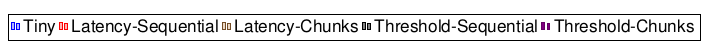
\includegraphics[scale=0.3]{images/legend}

    \subfloat[Yada]{
        \label{Yada}
        \begin{tikzpicture}[scale=0.35, baseline]
        \begin{axis}[
            width=1.5 \linewidth,
            height=1 \linewidth,
            %media de tempo intruder
            ybar=2.5pt,
            %enlargelimits=0.10,
            % legend style={at={(0.45,1.1)}, anchor=south, legend columns=-1},
            ylabel=Tempo(s),
            xlabel=Threads,
            symbolic x coords={1, 2, 4, 8, 16, 32, 64, 128, 256, 512},
            xtick=data,
            ymin=0,
            ymax=200,
            bar width=5pt,
            % nodes near coords,
            nodes near coords align={vertical},
        ]
        \addplot+[error bars,y dir=both, y explicit] coordinates {
            (1,9.95)+-(1,0.09) (2,19.42)+-(2,0.50) (4,15.05)+-(4,1.07) (8,12.75)+-(8,1.30) (16,8.85)+-(16,1.90) (32,15.25)+-(32,2.69) (64,18.85)+-(64,2.74) (128,51.34)+-(128,5.50) (256,89.66)+-(256,12.90) (512,189.43)+-(512,7.63) 
        };
        \addplot+[error bars,y dir=both, y explicit] coordinates {
            (1,14.09)+-(1,0.09) (2,9.88)+-(2,0.04) (4,7.22)+-(4,0.04) (8,4.78)+-(8,0.29) (16,4.19)+-(16,0.35) (32,4.74)+-(32,0.50) (64,5.38)+-(64,1.21) (128,12.38)+-(128,3.72) (256,13.14)+-(256,2.01) (512,15.43)+-(512,3.54)
        };
        \addplot+[error bars,y dir=both, y explicit] coordinates {
            (1,14.31)+-(1,0.16) (2,9.98)+-(2,0.07) (4,7.23)+-(4,0.11) (8,4.19)+-(8,1.93) (16,3.85)+-(16,0.97) (32,3.96)+-(32,1.37) (64,7.11)+-(64,1.83) (128,11.47)+-(128,2.48) (256,11.12)+-(256,5.94) (512,14.17)+-(512,1.47)
        };
        \addplot+[error bars,y dir=both, y explicit] coordinates {
            (1,14.17)+-(1,0.05) (2,14.17)+-(2,0.11) (4,14.20)+-(4,0.08) (8,11.61)+-(8,2.13) (16,13.53)+-(16,1.93) (32,15.15)+-(32,4.48) (64,14.19)+-(64,2.00) (128,15.69)+-(128,2.21) (256,27.92)+-(256,0.20) (512,22.18)+-(512,1.28) 
        };
        \addplot+[error bars,y dir=both, y explicit] coordinates {
            (1,14.35)+-(1,0.05) (2,14.29)+-(2,0.04) (4,14.31)+-(4,0.08) (8,14.31)+-(8,0.05) (16,15.07)+-(16,4.06) (32,13.64)+-(32,1.83) (64,6.83)+-(64,1.09) (128,13.37)+-(128,2.19) (256,15.65)+-(256,0.16) (512,15.73)+-(512,0.14)
        };
        % \legend {Tiny, Latency-Sequential, Latency-Chunks, Threshold-Sequential, Threshold-Chunks}
        \end{axis}
        \end{tikzpicture}
    }
\end{figure}

\end{frame}

\begin{frame} \frametitle{Aborts}
    \begin{block}{Aborts}
        gráficos
    \end{block}
\end{frame}

\section{Conclusão}
\begin{frame} \frametitle{Conclusão}
    \begin{block}{Analise}
        \begin{itemize}
        	\item Aplicações com conjunto pequeno de leitura e escrita;
        	\item Transação com tempo longo, médio, ou baixo;
        	\item Contenção alta, média ou baixa;
        	\item Redução de 96\% no tempo de execução; e
        	\item Redução de 99\% na ocorrencia de aborts.
        \end{itemize}
    \end{block}
\end{frame}

\begin{frame} \frametitle{Conclusão}
    \begin{block}{Trabalhos futuros}
        \begin{itemize}
        	\item Novas Heurísticas de distribuição;
        	\item Heurísticas de migração híbrida; e
        	\item Impacto energético dos escalonadores de STM.
        \end{itemize}
    \end{block}
\end{frame}

% \section{Objetivos}
% \begin{frame} \frametitle{Objetivos}
% \begin{block}{Objetivos}
% \begin{itemize}
% 	\item Estudar o comportamento dos escalonadores na arquitetura NUMA;
% 	\item Inserir as novas regras de escalonamento para arquitetura NUMA.
% \end{itemize}
% \end{block}
% \end{frame}

% \begin{frame} \frametitle{Metodologia}
%     \begin{block}{Ferramentas utilizadas}
%         \begin{itemize}
%         	\item Shrink;
%         	\item TinySTM;
%         	\item Hwloc; e
%         	\item STAMP.
%         \end{itemize}
%     \end{block}
% \end{frame}

% \begin{frame} \frametitle{Metodologia}
% \begin{block}{O que foi feito}
%     \begin{itemize}
%         \item Foi implementado um escalonador com filas de threads para cada núcleo;
%         \item Foi feito um escalonador que migra threads;
%     	\item Foram estudados os algoritmos de escalonamentos atuais; e
%     	\item Foi desenvolvido um novo fluxo de execução para o Shrink.
%     \end{itemize}
% \end{block}
% \end{frame}

% \begin{frame} \frametitle{Metodologia}
% \begin{block}{O que será feito}
% \begin{itemize}
% 	\item Modificar a implementação de threads do Shrink para utilizar filas;
% 	\item Coletar informações da latência de acordo com o Bloom Filter; e
% 	\item Adicionar a migração de threads ao Shrink.
% \end{itemize}
% \end{block}
% \end{frame}

% \begin{frame} \frametitle{Metodologia}
% \begin{block}{Modificações e nomenclatura}
% \begin{itemize}
% 	\item Cada núcleo possuirá uma fila de threads que chamamos de Qn;
% 	\item O escalonador possuirá uma fila de threads inicial chamada de Pt; e
% 	\item Uma Thread (Tn) pode ter n transações que chamamos de Tr.
% \end{itemize}
% \end{block}
% \end{frame}

% \begin{frame} \frametitle{Metodologia}
%     \begin{figure}[!h]
% 	    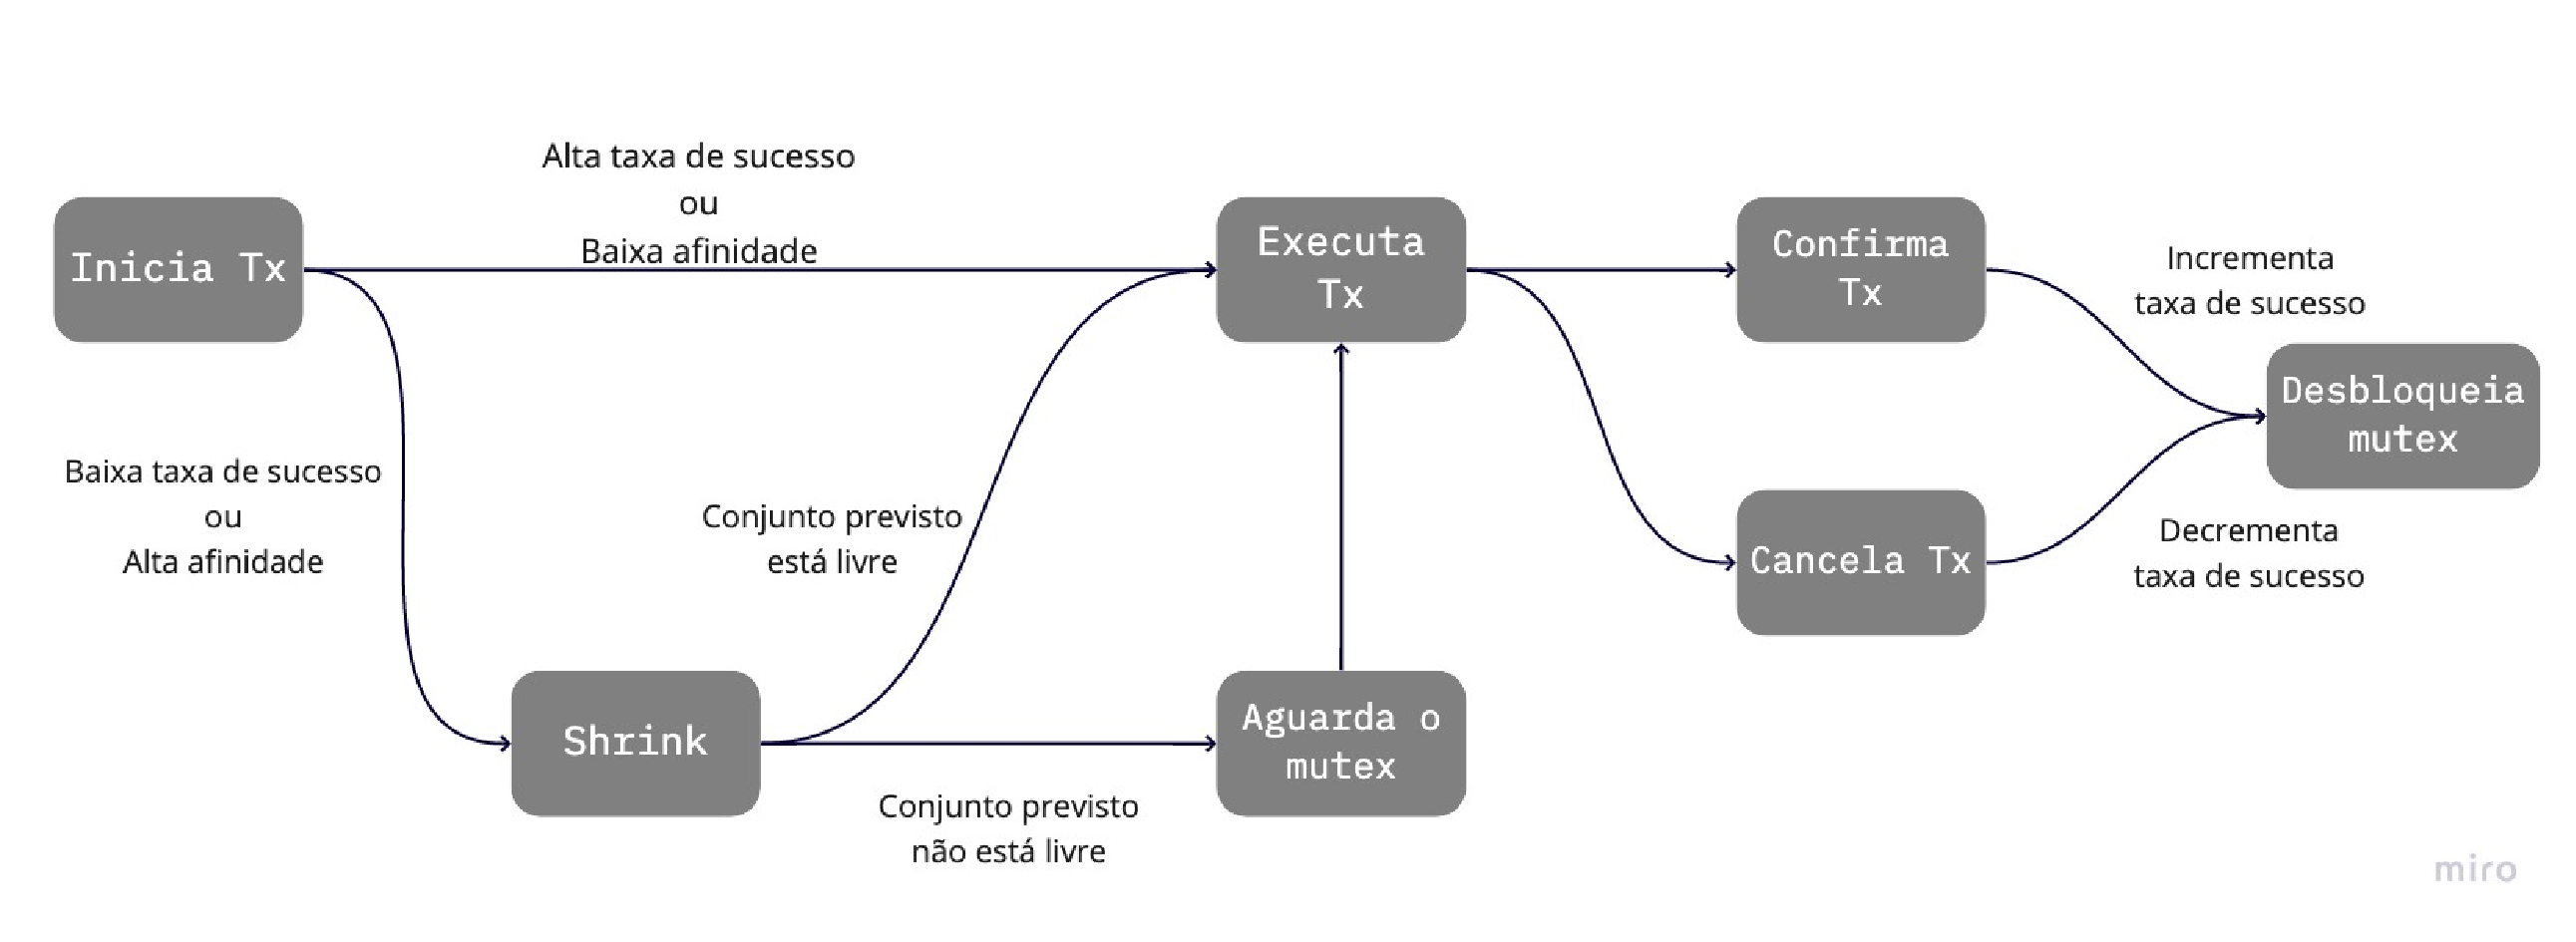
\includegraphics[scale=0.25]{images/ShrinkFlow}
% 	    \caption{Shrink}
% 	    \label{fig:abusy}
%     \end{figure}
% \end{frame}

% \begin{frame} \frametitle{Metodologia}
%     \begin{figure}[!h]
% 	    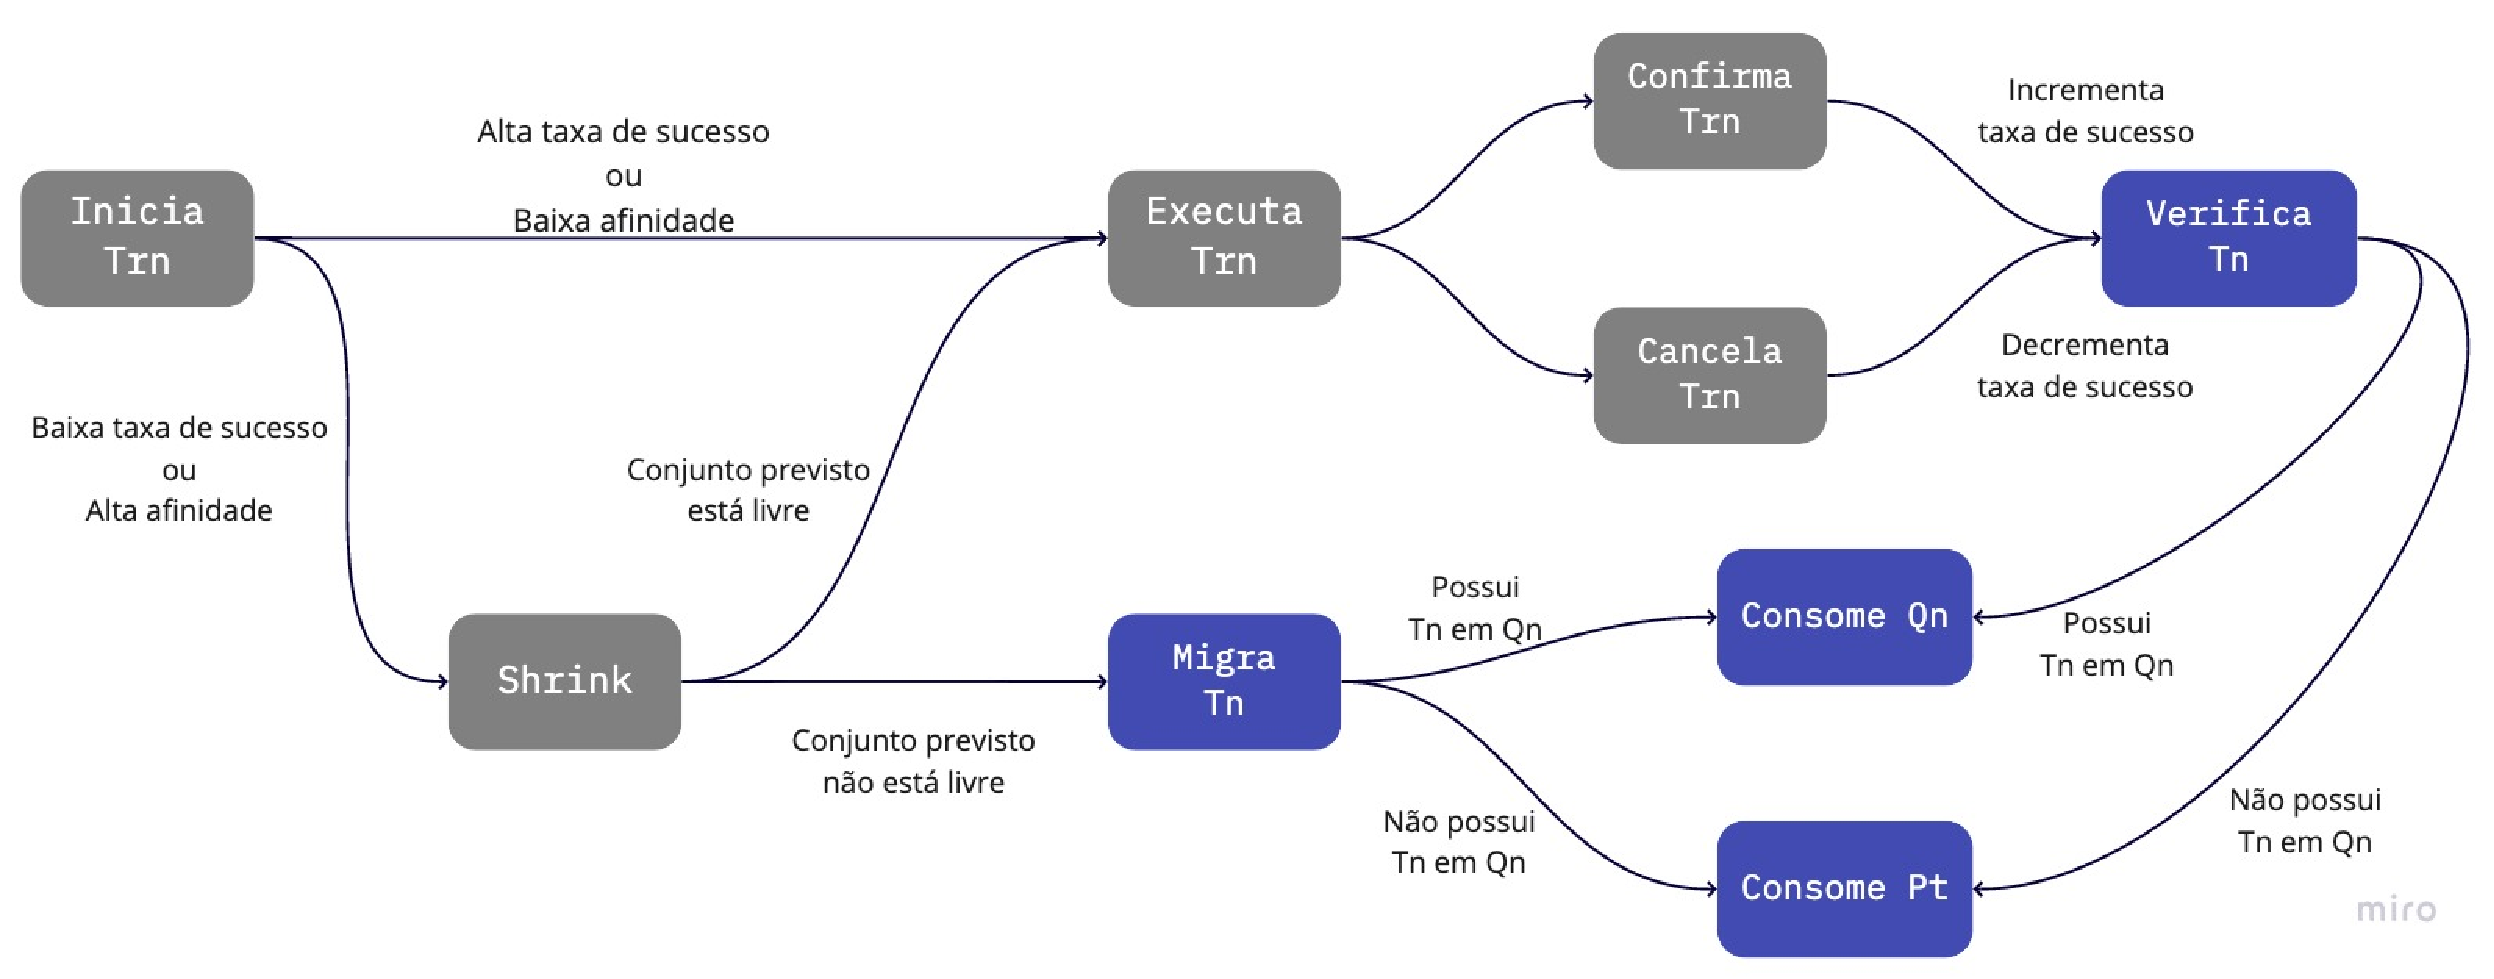
\includegraphics[scale=0.25]{images/LScheduleFlow}
% 	    \caption{Modificações}
% 	    \label{fig:abusy}
%     \end{figure}
% \end{frame}

% \section{Próximas Atividades}
% \begin{frame} \frametitle{Próximas Atividades}
% \begin{block}{Atividades a serem realizadas}
% \begin{itemize}
% 	\item Modificar o escalonador Shrink;
% 	\item Executar os testes;
% 	\item Analisar resultados; e
% 	\item Escrever a Dissertação.
% \end{itemize}
% \end{block}
% \end{frame}

% \section{Cronograma de Atividades}

% \begin{frame} \frametitle{Cronograma}
% \begin{enumerate}
% 	\item Modificações no Shrink coletando informações sobre a arquitetura;
% 	\item Modificações no método de escalonamento do Shrink;
% 	\item Validação do novo método de escalonamento;
% 	\item Execução de testes em arquitetura NUMA e UMA;
% 	\item Coleta de resultados obtidos por meio dos testes;
% 	\item Escrita da dissertação; e
% 	\item Entrega e apresentação da dissertação.
% \end{enumerate}
% \end{frame}

% \begin{frame} \frametitle{Cronograma}
% \begin{table}[!h]
% \centering
% \caption{Cronograma de atividades mensal para o restante do mestrado}
% \label{tab:cro2}
% \scalebox{0.75}{
% 	\begin{tabular}{c|c|c|c|c|c|c|c} \hline
% 		Ano & \multicolumn{5}{|c|}{2020} & \multicolumn{2}{|c}{2021} \\ \hline
% 		Mês & Ago & Set & Out & Nov & Dez & Jan & Fev \\ \hline
% 		1   & \tn & \tn & \tn & &   &   &   \\ \hline
% 		2   &   & \tn & \tn & \tn & &   & \\ \hline
% 		3   &   &   &   & \tn & \tn & &   \\ \hline
% 		4   &   &   &   &   & \tn & \tn & \\ \hline
% 		5   &   &   &   &   & & \tn &  \tn \\ \hline
% 		6   &   & \tn & \tn & \tn & \tn & \tn & \tn \\ \hline
% 		7   &   &   & &   & & & \tn \\ \hline	
% \end{tabular}
% }
% \end{table}
% \end{frame}
\maketitle
\end{document}

